
\section{Vektorer og linjer i planen}
\emph{Forklar om vektorer i planen.}

En vektor er en pil, der har en retning og en vektor.

Når vi regner med vektorer, så anvender vi kartesisk notation.

Nemt at lave vektorer mellem punkter, da kartesisk notation præcis er $\Delta x$ og $\Delta y$.

Man kan skalere en vektor ved at gange begge koordinater af en vektor.

Skalarproduktet, der er ikke gange eller dividere, er defineret
som $\vec{x}\cdot \vec{y}=x_1 \cdot y_1+x_2 \cdot y_2$.

Når 2 vektorer er ortogonale, hvilket vil sige, at de danner en
90 graders vinkel, så er skalarproduktet 0.

\subsection{Bevis af linjens parameterfremstilling}

\begin{proofw}
    Betragt følgende skitse:
    \begin{figure}[h]
        \centering
        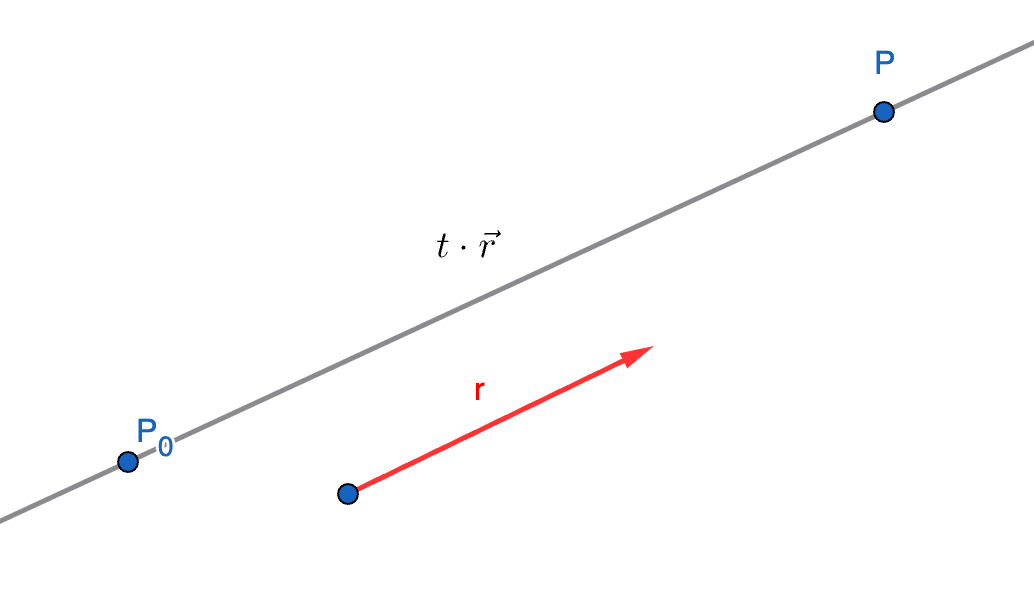
\includegraphics[scale=0.4]{skitser/linje_parameter.png}
    \end{figure}

Tager vi afsæt i punktet $P_0(x_0,y_0)$, hvis position kan beskrives
med vektoren $\vec{OP}$. Tager vi et skridt langs en vektor, der er parallel med linjen,
så vil vores nye position også være på linjen.
Derfor må vi ved at gange retningsvektoren med et vilkårligt tal
kunne ramme alle punkter på linjen.
Så kan vi beskrive vektoren til punktet $P(x,y)$
som vektoren til $P_0$ plus retningsvektoren skaleret:

$$
\vec{OP}=\vec{OP_0}+t\cdot \vec{r}
$$

Vi opsplitter $\vec{OP}$ i $\begin{pmatrix}
    x \\ y
\end{pmatrix}$ og $\vec{r}$ i $\begin{pmatrix}
    r_1 \\ r_2
\end{pmatrix}$:

$$
\begin{pmatrix}
    x
    \\
    y
\end{pmatrix}
=\begin{pmatrix}
    x_0
    \\
    y_0
\end{pmatrix}
+
t \cdot \begin{pmatrix}
    r_1
    \\
    r_2
\end{pmatrix}
$$
\end{proofw}

\subsection{Bevis af linjens ligning}

\begin{proofw}
    Betragt nedenstående figur:
    \begin{figure}[h]
        \centering
        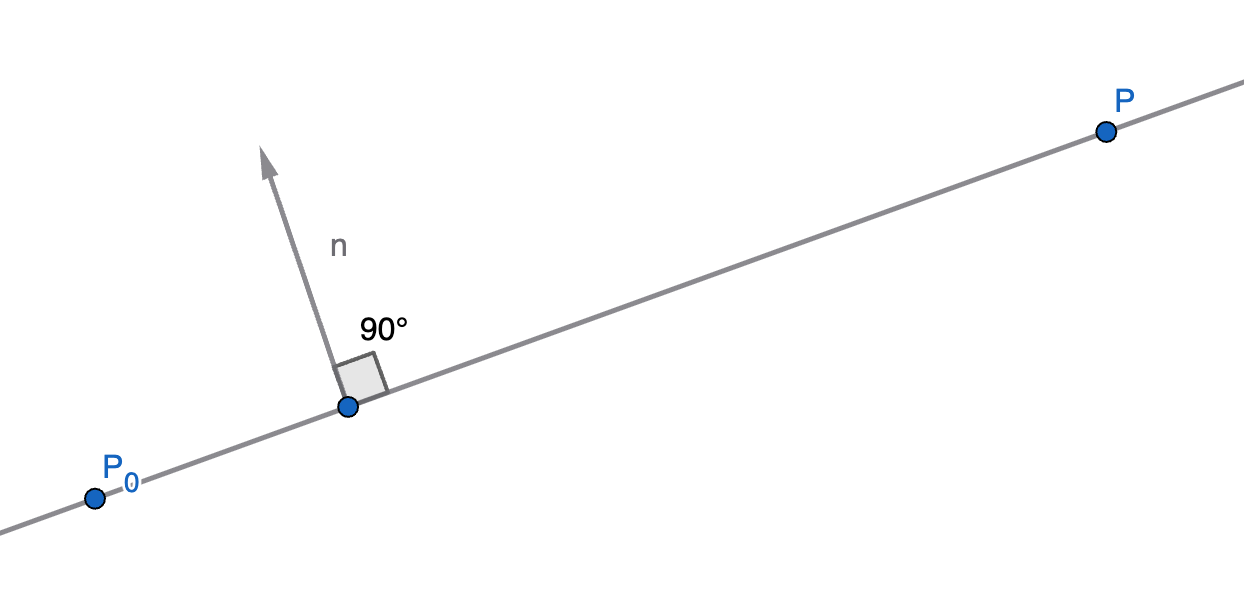
\includegraphics[scale=0.4]{skitser/linjens_ligning.png}
    \end{figure}

    Vi kender $P_0(x_0,y_0)$ og normalvektoren $\vec{n}=\begin{pmatrix}
        a \\ b
    \end{pmatrix}$, $P(x,y)$ er et vilkårligt punkt langs linjen, som vi vil beskrive.
    Vi kan lave en ortogonal vektor til $\vec{n}$ ved at lave vektoren $\vec{P_0P}=\begin{pmatrix}
        x-x_0
        \\
        y-y_0
    \end{pmatrix}$.
    Tricket er så, at vi har 2 ortogonale vektorer, hvilket betyder,
    at deres skalarprodukt er 0, derved kan vi opstille følgende udtryk, hvor $x$ og $y$ alle er punkter på linjen:

    \begin{align*}
        \vec{P_0P}&\cdot\vec{n}=0
        \\
        &\Downarrow
        \\
        \begin{pmatrix}
            x-x_0
            \\
            y-y_0
        \end{pmatrix}
        &\cdot
        \begin{pmatrix}
            a \\
            b
        \end{pmatrix}=0
        \\
        \Downarrow
        \\
        a(x-x_0)&+b(y-y_0)=0
        \\
        \Downarrow
        \\
        ax+by+&(-ax_0-by_0)=0
        \\
        \Downarrow
        \\
        ax+by&+c=0
    \end{align*}

    Det er vist, at en linje kan beskrives ud fra et punkt og en normalvektor til linjen.

\end{proofw}
